\section{Explosions: particles, physics and colour}
\label{sec:explode}
An explosion is a particle system: one call spawns a few hundred short-lived
particles of seven kinds, each with a position, velocity, size, life and heat. Every tick each particle is moved by
its own simple law of motion (Table~\ref{tab:explode}); every frame each one is drawn as a single instanced quad --- the
$+Z$ face of the unit cube --- turned to face the camera (puffs), stretched along its velocity (sparks, embers),
or laid flat on the ground (shock wave, scorch). Its colour is not stored anywhere: the fragment shader computes it
from a temperature $T$.
\begin{table}[H]
\centering\footnotesize\setlength{\tabcolsep}{3pt}
\explosiontable
\caption{What one blast spawns (power 1 = a UAV round, 1.6 = a tank shell, 0.15 = a tracer impact), how each kind
moves per tick of length $\Delta t$ and how its colour is made.}
\label{tab:explode}
\end{table}

\paragraph{Physics.} All drag terms are exact exponential decays, $\mathbf{v}\leftarrow\mathbf{v}\,e^{-k\Delta t}$,
so a puff slows the same way at 30 or 144\,fps (a factor $(1-k\Delta t)$ would not). Hot gas has positive buoyancy
(fire $+\gv{fireRise}$\,m/s$^2$, smoke $+\gv{smokeRise}$\,m/s$^2$ capped at \gv{smokeMaxUp}\,m/s) and smoke relaxes towards the wind velocity; sparks
fall with $g=\gv{gravity}$\,m/s$^2$ and bounce off the terrain keeping $\gv{bounce}$ of their vertical speed. Smoke grows as it rises
(size $+\,$growth$\cdot e^{-\gv{smokeGrowK}\,\mathrm{age}}$), which is what turns the fireball into a column. The destroyed rover is not
replaced by a model of a wreck: its own primitives (Section~\ref{sec:decomp}) become rigid debris pieces, thrown away from the
blast with speed $\propto\sqrt{\text{power}}$, spinning about a random axis, integrated in sub-steps of
1/\gv{debrisSub}\,s with restitution \gv{debrisRest}, sliding friction \gv{debrisFric}, and put to rest below
\gv{debrisRestSpeed}\,m/s; their materials are charred (albedo $\times0.1$, roughness 0.95) and start hot in the thermal image.
\begin{figure}[H]
\centering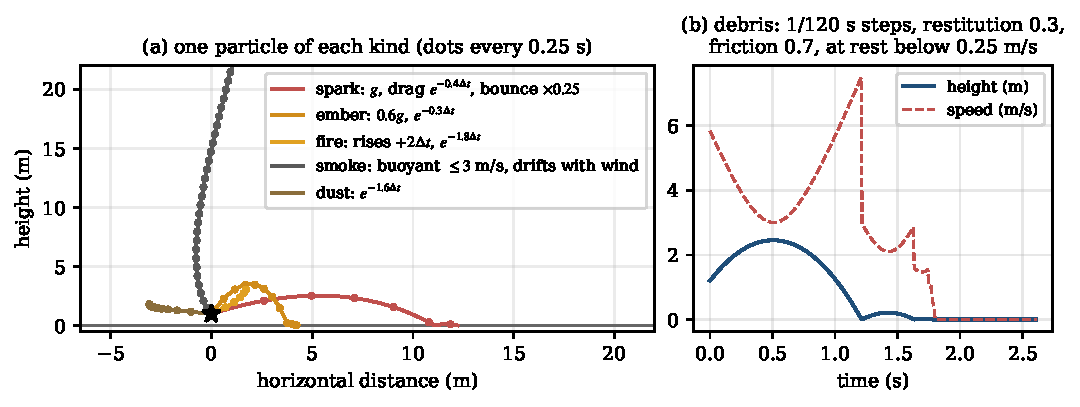
\includegraphics[width=\linewidth]{figures/diagrams/d_particles.pdf}
\caption{The integrators of Table~\ref{tab:explode} run from the same start point (initial velocities are typical
spawn values); (b) one debris piece bouncing to rest.}
\label{fig:particles}
\end{figure}

\paragraph{Colour from temperature.} A flame quad does not use a texture. The shader builds a temperature field from
fractal noise that scrolls upwards, $T=\mathrm{clamp}(1-d)\,(1-t)^{\gv{fireLife}}$ ($d$ = noisy distance from the
centre, $t$ = age/life), and maps it to colour with a blackbody-like ramp in which red rises first, then green, then
blue:
\begin{equation}
\mathrm{bb}(T)=\big(T^{\gv{bbR}},\ T^{\gv{bbG}},\ \gv{bbBk}\,T^{\gv{bbB}}\big),\qquad
\mathbf{c}_{\mathrm{fire}}=\mathrm{bb}(T)\,(\gv{fireEmitA}+\gv{fireEmitB}\,T^2)
\label{eq:bb}
\end{equation}
so a cooling point slides continuously from white-yellow through orange and deep red to black --- colour
interpolation along a curve through RGB space rather than a straight line between two colours. The emission is in
HDR (the core is several times brighter than 1), so bloom and the tone mapper of Section~\ref{sec:color} make it glow.
Sparks cool along the same ramp, $T_n=h(1-\gv{sparkCool}\,t)$; smoke is a lit, noise-eroded volume whose underside
keeps a warm glow $(\gv{smokeGlowR},\gv{smokeGlowG},\gv{smokeGlowB})\,e^{-\gv{smokeGlowDecay}\,\mathrm{age}}$ from the fire below it; the flash mixes orange
into white towards its centre. Blending is premultiplied ($\mathrm{src}+(1-\alpha)\,\mathrm{dst}$, depth writes off): emission adds light,
alpha (soot, smoke) hides what is behind. Two instanced draws per frame: first the smoke and dust group, then the
glowing group (fire, sparks, flash), each sorted back to front by distance to the camera. In the thermal
view the same particles write heat instead of colour; smoke cools as $h=\gv{smokeHeatFloor}+(h_0-\gv{smokeHeatFloor})\,e^{-\gv{smokeHeatK}\,\mathrm{age}}$.
\begin{figure}[H]
\centering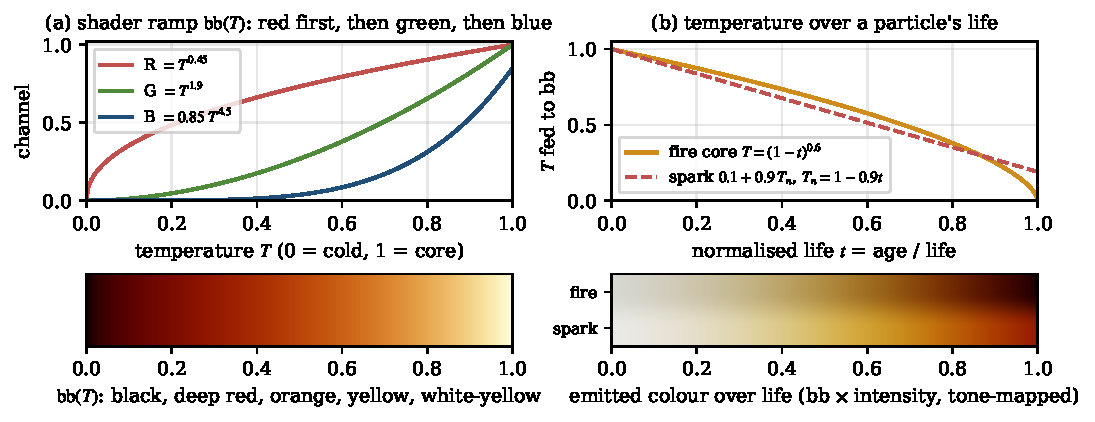
\includegraphics[width=\linewidth]{figures/diagrams/d_blackbody.pdf}
\caption{(a) The shader's ramp (Eq.~\ref{eq:bb}) per channel and as a colour bar; (b) the temperature a flame core
and a spark feed into it over their lives, and the resulting emitted colour (HDR, shown tone-mapped).}
\label{fig:bb}
\end{figure}
\begin{figure}[H]
\centering
\wbblock{Explosion}{bb}\\[1.5mm]
\wbblock{Explosion}{life}\\[1.5mm]
\begin{minipage}[t]{0.5\linewidth}\centering\wbblock{Explosion}{spark}\end{minipage}\hfill
\begin{minipage}[t]{0.46\linewidth}\centering\wbblock{Explosion}{debris}\end{minipage}\\[1mm]
{\footnotesize\wbkey}
\caption{Workbook sheet \code{Explosion}: the colour ramp and the fire emission factor per temperature, the colour of a
flame core and a spark over their lives, one spark integrated step by step, and the debris bounce series. \fullsheet{Explosion}}
\label{fig:wb-explosion}
\end{figure}
\begin{figure}[H]
\centering
\begin{subfigure}{0.245\linewidth}\raw{game/explosion_early}{\linewidth}\caption{Flash and fireball.}\end{subfigure}\hfill
\begin{subfigure}{0.245\linewidth}\raw{game/explosion_mid}{\linewidth}\caption{Fire cools, sparks fall.}\end{subfigure}\hfill
\begin{subfigure}{0.245\linewidth}\raw{game/explosion_smoke}{\linewidth}\caption{5\,s on: the next round's flash.}\end{subfigure}\hfill
\begin{subfigure}{0.245\linewidth}\raw{game/wreck_burning}{\linewidth}\caption{Burning wreck.}\end{subfigure}
\caption{One blast over time; the fire's colour moves along the ramp of Figure~\ref{fig:bb} as it cools.}
\label{fig:boom}
\end{figure}
In Figure~\ref{fig:boom}a the flash and sparks are white-yellow with the shock-wave ring; in (b) the fire turns orange
and deep red as it cools; in (c) a second round's flash is white again while the first blast burns low and red.

\textbf{Limitation.} Sorting is per group, not across the two groups: a glowing particle behind a smoke puff is drawn after
the puff and so shows through it (bright additive light makes this hard to notice). Sparks and embers bounce on
the terrain only, not on buildings.
